%----------------------------------------------
% PACCHETTI
%----------------------------------------------
\documentclass[12pt,a4paper]{article}
\usepackage[a4paper]
\usepackage[T1]{fontenc}
\usepackage[utf8]{inputenc}
\usepackage[italian]{babel}
\usepackage{lipsum}
\usepackage{hyperref}
\usepackage{lastpage}
\usepackage{fancyhdr}
\usepackage{graphicx}
\usepackage{url}
\usepackage{geometry}
\usepackage{xcolor}
\usepackage{amssymb}
\usepackage{amsmath}
\usepackage{booktabs}

%----------------------------------------------
% NUOVI COMANDI
%----------------------------------------------
\newcommand{\Sep}{\vspace{1.5em}}
\newcommand{\MidSep}{\vspace{1em}}
\newcommand{\SmallSep}{\vspace{0.5em}}

\newcommand{\numberset}{\mathbb}
\newcommand{\N}{\numberset{N}} 
\newcommand{\Z}{\numberset{Z}}
\newcommand{\Q}{\numberset{Q}}
\newcommand{\R}{\numberset{R}}
\newcommand{\C}{\numberset{C}}
%----------------------------------------------
% INTESTAZIONE  E PIE DI PAGINA
%----------------------------------------------
\pagestyle{myheadings}
\pagestyle{fancy}
\fancyhf{}
\hypersetup{hidelinks}

\headsep= 20mm

\renewcommand{\headrulewidth}{2pt}
\renewcommand{\footrulewidth}{2pt}

\lhead{
\includegraphics[width=0.4\columnwidth]{img/units_logo}}
\rhead{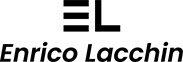
\includegraphics[width=0.3\columnwidth]{img/logo_black}}\lfoot{© Enrico Lacchin | \url{www.enricolacchin.com}}
\cfoot{}
\rfoot{\thepage}

\leftskip 0.0pt
\usepackage[utf8]{inputenc}
\usepackage{amsmath}
\usepackage{amssymb}
\usepackage{xcolor}
\usepackage{listings}
\usepackage{xstring}

\definecolor{dkgreen}{rgb}{0,0.6,0}
\definecolor{ltgray}{rgb}{0.5,0.5,0.5}
\definecolor{royalpurple}{rgb}{0.47, 0.32, 0.66}

\makeatletter
\newif\ifcolname
\colnamefalse

\def\keywordcheck{%
\IfStrEq*{\the\lst@token}{SELECT}{\global\colnametrue}{}%
\IfStrEq*{\the\lst@token}{WHERE}{\global\colnametrue}{}%
\IfStrEq*{\the\lst@token}{FROM}{\global\colnamefalse}{}%
\IfStrEq*{\the\lst@token}{USE}{\global\colnamefalse}{}%
\color{orange}%
}
\def\setidcolor{%
\ifcolname\color{royalpurple}\else\color{black}\fi%
}
\makeatother

\lstset{
    basicstyle={\small\ttfamily},
    breakatwhitespace=false,
    breaklines=true,
    captionpos=b,
    commentstyle=\color{dkgreen},
    deletekeywords={...},
    escapeinside={\%*}{*)},
    extendedchars=true,
    frame=single,
    keepspaces=true,
    language=SQL,
    otherkeywords={IS, IF, SHOW, DECLARE, OPEN, FETCH, CLOSE, DATABASE, DATABASES, USE, COMMENT, CHANGE, REFERENCES, RENAME, TO, IS, AUTO_INCREMENT, EXISTS},
    morekeywords={*,modify,MODIFY,...},
    keywordstyle=\keywordcheck,
    identifierstyle=\setidcolor,
    stringstyle=\color{red},
    numbers=left,
    numbersep=15pt,
    numberstyle=\tiny,
    rulecolor=\color{ltgray},
    showspaces=false,
    showstringspaces=false, 
    showtabs=false,
    stepnumber=1,
    tabsize=2,
    xleftmargin =1em
}

%----------------------------------------------
% INIZIO DOCUMENTO
%----------------------------------------------
\begin{document}
\setlength{\parindent}{0cm}

%----------------------------------------------
% TITOLO
%----------------------------------------------
\pagenumbering{gobble}

\small{Enrico Lacchin}

\MidSep
\textbf{\LARGE{Basi di Dati}}

\MidSep
\textit{\Large{Appunti}}
\Sep

\begin{center}
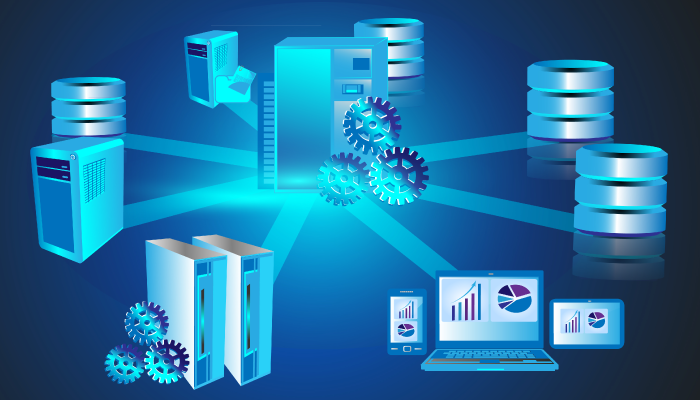
\includegraphics[width=1\columnwidth]{img/database.png}
\end{center}

\vfill
Materia: Basi di Dati

Docente: Andrea De Lorenzo

Pagina corso: \url{http://delorenzo.inginf.units.it/project/basi-di-dati-2023/}

%----------------------------------------------
% INDICE
%----------------------------------------------

\clearpage
\pagenumbering{roman}
\setcounter{page}{1}
\tableofcontents

%----------------------------------------------
% INIZIO CAPITOLI
%----------------------------------------------
%CAPITOLO 1
\clearpage

\pagenumbering{arabic}
\setcounter{page}{1}

%CAPITOLO 1
\section{Introduzione}
\subsection{Gestione delle informazioni}
L'essere umano genera e gestisce tante informazioni:
\begin{itemize}
\item Idee informali
\item Linguaggio naturale
\item Disegni, grafici, schemi
\item Numeri
\item Codici
\end{itemize}
e vengono salvate in tanti modi diversi
\begin{itemize}
\item Memoria
\item Carta
\item Pietra
\item Scritta sul muro
\item Elettronica
\end{itemize}

\SmallSep \noindent
Anche le organizzazioni generano informazioni:
\begin{itemize}
\item Utenze telefoniche
\item Conti correnti
\item Studenti iscritti ad un corso di laurea
\item Quotazioni di azioni
\end{itemize}

\subsection{Informazione vs Dato}
\textbf{Informazione}: notizia, dato o elemento che consente di avere conoscenza più o meno esatta di fatti, situazioni, modi di essere.\\
\textbf{Dato}: elemento di informazione costituito da simboli che debbono essere elaborati.\\

\subsection{Numeri}
\begin{center}Come codifico i numeri?\end{center}
Numeri naturali: in binario\\
Numeri interi: devo decidere come rappresentare il segno\\
Numeri razionali? 10010011110011001111

\subsection{Dati e Applicazioni}
I \textbf{dati} possono variare nel tempo. Le \textbf{modalità} con cui i dati sono rappresentati sono di solito stabili. Le \textbf{operazioni} sui dati variano spesso.\\
\begin{center}\textbf{\'E importante separare i dati dalle applicazioni che operano su essi}\end{center}

\subsection{Database}
\textbf{Genericamente}: Collezione di dati, utilizzati per rappresentare le informazioni di interesse per una o più applicazioni di una organizzazione.
\begin{itemize}
\item Schede perforate
\item File CSV
\item Foglio di calcolo
\item File XML
\item Access
\end{itemize}

\SmallSep \noindent
\textbf{Per noi}: Collezione di dati gestita da un DBMS (\ref{DBMS})

\subsection{Database Management System [DBMS]}\label{DBMS}
Un DMBS è un software in grado di gestire collezioni di dati che siano:
\begin{itemize}
\item \textbf{Grandi}: di dimensioni (molto) maggiori della memoria centrale
\item \textbf{Persistenti}: con un periodo di vita indipendente dalla singole esecuzioni dei programmi che le utilizzano
\item \textbf{Condivise}: utilizzate da applicazioni diverse
\end{itemize}
Un DBMS deve garantire:
\begin{itemize}
\item \textbf{Affidabilità}: resistenza a malfunzionamenti hardware e software
\item \textbf{Privatezza}: con una disciplina e un controllo degli accessi
\item \textbf{Efficienza}: utilizzando al meglio le risorse di spazio e tempo del sistema
\item \textbf{Efficacia}: rendendo produttive le attività dei suoi utilizzatori
\end{itemize}

\paragraph{Condivisione\\}
L’integrazione e la condivisione permettono di
\begin{itemize}
\item Ridurre la \textsl{ridondanza} (evitando ripetizioni)
\item Ridurre possibilità di incoerenza (o \textsl{inconsistenza}) fra dati
\end{itemize}
Poiché la condivisione non è mai completa (o comunque non opportuna) i DBMS prevedono meccanismi per
\begin{itemize}
\item \textsl{Privatezza} dei dati
\item Limitazione all'accesso (\textsl{autorizzazioni})
\end{itemize}
La condivisione richiede coordinamento degli accessi: \textsl{controllo della concorrenza}

\paragraph{Efficienza\\}
Si misura in termini di tempo di esecuzione e spazio di memoria (principale e secondaria)\\
I DBMS non sono necessariamente più efficienti dei file system\\
L’efficienza è il risultato della qualità del DBMS e delle applicazioni che lo utilizzano

\subsubsection{DBMS vs FS}
\begin{center}\resizebox{0.6\columnwidth}{!}{%
\begin{tabular}{|l|c|c|} \hline
 & DBMS & FS \\ \hline
Grandi moli di dati & \checkmark & \checkmark \\ \hline
Persistenti & \checkmark  & \checkmark \\ \hline
Condivisi & \checkmark & \checkmark \\ \hline
Affidabile & \checkmark & \checkmark \\ \hline
Privatezza & \checkmark & \checkmark \\ \hline
Efficienza & ? & ? \\ \hline
Efficacia & X & \checkmark \\ \hline
\end{tabular}}\end{center}

\subsection{File System}
Descrizione dei dati contenuta nell'applicazione
\begin{center}
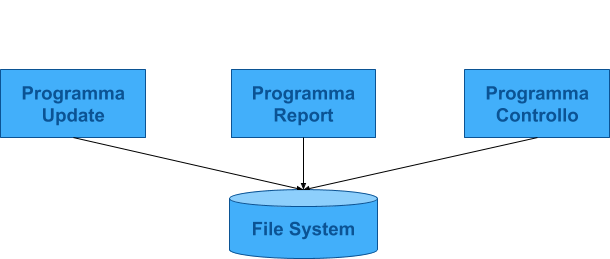
\includegraphics[width=0.6\columnwidth]{img/file_system.png}
\end{center}
In un FS se si va a modificare una delle applicazioni, le altre applicazioni collegate vanno in crash
\begin{center}
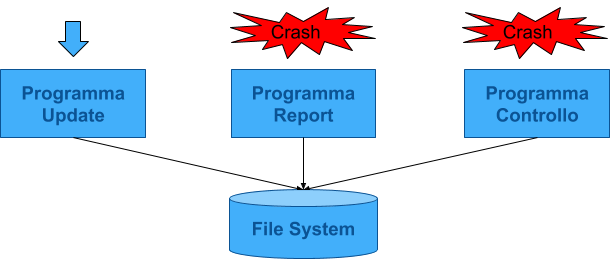
\includegraphics[width=0.6\columnwidth]{img/file_system2.png}
\end{center}

\paragraph{DBMS e Descrizione dei dati\\}
Il DBMS sa come persistere i dati, per l’applicazione è un atto di fede. I dati sono INDIPENDENTI dalla forma fisica. I programmi parlano con il DBMS per accedere ai dati

\subsection{Modello Concettuale}
Il modello concettuale non dipende dallo strumento utilizzato\\
\begin{center}Analisi del problema $\Longrightarrow$ Modello astratto\end{center}

\subsection{Modello Logico}
Il modello logico indica come rappresentare i dati individuati con il modello concettuale. 
\begin{itemize}
\item Livello intermedio tra utente e implementazione
\item Sottintende una specifica rappresentazione dei dati (tabelle, alberi, grafi, oggetti, …)
\end{itemize}

\subsection{Database System}
Un database system è formato da:
\begin{itemize}
\item \textbf{Software}:
\begin{itemize}
\item DBMS: interposto tra il DB e l'utente
\item Utility di supporto (sviluppo, backup)
\end{itemize}
\item \textbf{Utenti}:
\begin{itemize}
\item Progettista
\item Sviluppatore
\item Amministratore
\item Utente finale
\end{itemize}
\item \textbf{Schemi} (struttura dei dati)
\item \textbf{Dati}:
\begin{itemize}
\item Come vengono salvati
\item Condivisione
\item Concorrenza
\item Ridondanza
\end{itemize}
\item \textbf{Hardware}
\end{itemize}

\subsubsection{Vantaggi e Svantaggi}
\textcolor{gg}{\textbf{Vantaggi}}:
\begin{itemize}
\item Dati sono risorsa in comune
\item DB fornisce un modello unificato del business
\item Controllo centralizzato dei dati, quindi standardizzazione ed economie di scala
\item Riduzione ridondanza ed inconsistenza
\item Indipendenza dei dati
\end{itemize}
\textcolor{red}{\textbf{Svantaggi}}:
\begin{itemize}
\item Costo e complessità
\item Servizi ridondanti/non necessari
\end{itemize}

\subsection{Schema ed Istanza}
In ogni database e esistono:
\begin{itemize}
\item \textbf{Schema}:
\begin{itemize}
\item Invariante nel tempo
\item Descrive la struttura
\item eg: intestazione tabelle
\end{itemize}
\item \textbf{Istanza}:
\begin{itemize}
\item I valori attuali
\item Possono cambiare
\item eg: contenuto delle tabelle
\end{itemize}
\end{itemize}

%CAPITOLO 2
\clearpage
\section{Schemi}
\begin{center}
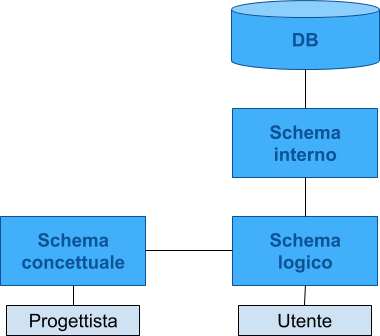
\includegraphics[width=0.6\columnwidth]{img/schemi.png}
\end{center}
\paragraph{Schemi concettuali}
Permettono di rappresentare i dati in modo indipendente da ogni sistema:
\begin{itemize}
\item Cercando di descrivere i concetti del mondo reale
\item Sono utilizzati nelle fasi preliminari di progettazione
\end{itemize}
Modello più diffuso: \textbf{Entity-Relationship}

\subsection{Schemi interni (o fisici)}
Rappresentazione dello schema logico per mezzo di strutture di memorizzazione
\begin{itemize}
\item File CSV
\item File XML
\item File binari
\end{itemize}

\subsection{Schemi logici}
Com'è organizzato il DB? Diverse soluzioni:
\begin{itemize}
\item Gerarchico
\item Reticolare
\item Relazionale
\item Ad oggetti
\end{itemize}
\textbf{Indipendenza}
Lo schema logico è indipendente da quello fisico.\\
ES: una tabella è utilizzata sempre allo stesso modo qualunque sia la sua realizzazione fisica (che può variare nel tempo)
\begin{center}\textbf{PROGETTISTA DB $\not =$ SVILUPPATORE SW}\end{center}

\subsection{Vista}
L'amministratore del DB può modificare la struttura interna dei dati senza toccarne la visibilità esterna $\Longrightarrow$ Immunità delle applicazioni a modifiche di struttura
\begin{center}\textbf{SCHEMA ESTERNO $=$ VISTA}\end{center}
\begin{itemize}
\item Descrive parte della base di dati di un modello logico
\item NON è una copia dei dati
\end{itemize}

\subsubsection{Architettura ANSI/SPARC}
\begin{center}
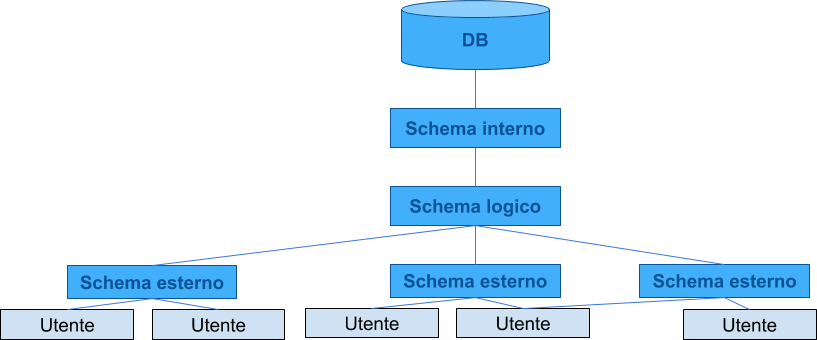
\includegraphics[width=0.6\columnwidth]{img/ansisparc.png}
\end{center}

\subsection{Schemi logici}
\begin{center}
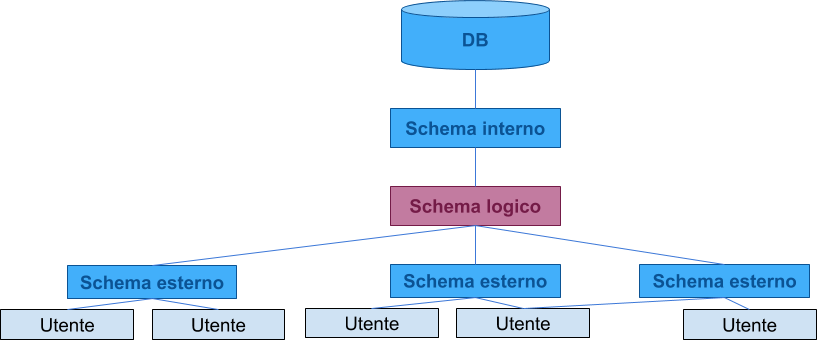
\includegraphics[width=0.6\columnwidth]{img/logici.png}
\end{center}

\subsection{Schemi logici gerarchici}
\begin{center}
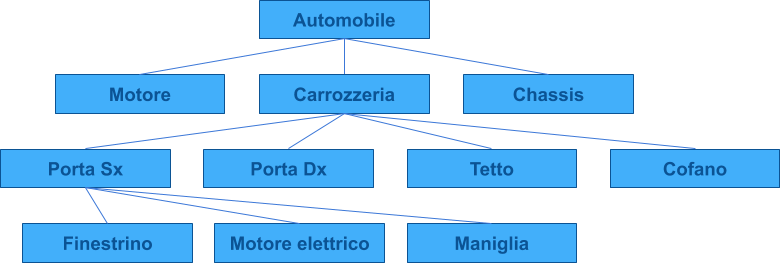
\includegraphics[width=0.6\columnwidth]{img/gerarchico.png}
\end{center}
\textbf{Problemi}:
\begin{itemize}
\item Accesso sequenziale: per arrivare al figlio devo attraversare tutti i nodi
\item Modifica parziale complicata
\item Cancellazione gerarchica
\item Stretto legame tra programma e struttura del database
\item Ridondanza
\end{itemize}

\subsection{Schemi logici gerarchici (ridondanza)}
\begin{center}
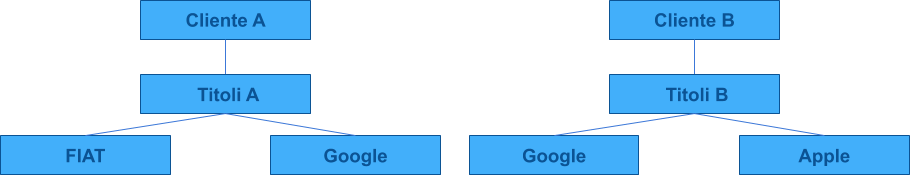
\includegraphics[width=0.6\columnwidth]{img/ridondanza.png}
\end{center}

\subsection{Schemi logici reticolari}
\begin{center}
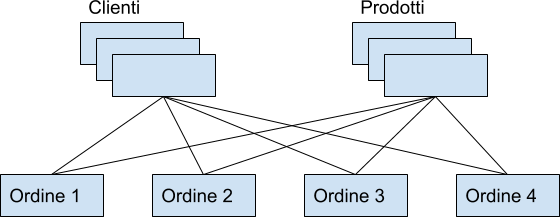
\includegraphics[width=0.6\columnwidth]{img/reticolare.png}
\end{center}
\begin{itemize}
\item COBOL, 1970
\item Nodi collegati da puntatori
\item Navigazione bi-direzionale
\end{itemize}
\begin{center}
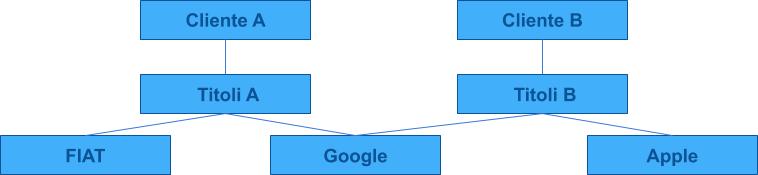
\includegraphics[width=0.6\columnwidth]{img/ridondanzaok.png}
\end{center}

\subsection{Schemi logici relazionali} 
[CODD, 1980]\\
L'obiettivo di questi schemi è quello di liberarsi dai puntatori fisici
\begin{itemize}
\item I dati sono organizzati in tabelle di valori
\item Le operazioni vengono eseguite sulle tabelle
\item I risultati delle operazioni sono tabelle
\item I riferimenti tra dati in strutture (tabelle) diverse sono rappresentati con valori
\end{itemize}

\subsubsection{Elementi di un DBR}
\textbf{Tabelle}: organizzazione rettangolare di dati
\begin{itemize}
\item Record (righe) e campi (colonne) e domini dei dati
\item I campi definiscono univocamente il tipo dei dati (dominio)
\item I campi hanno un nome ed un ordine, le righe no
\item Esistono tabelle vuote
\end{itemize}

\paragraph{Chiavi Primarie [PK]\\}
\begin{itemize}
\item Una (o più) colonne che identificano \textbf{UNIVOCAMENTE} il record
\item Non possono essere duplicate
\item Una tabella in cui ogni riga è diversa dalle altre è detta \textbf{RELAZIONE}
\end{itemize}

\paragraph{Relazioni\\}
\begin{itemize}
\item Non esistono relazioni padre-figlio
\item Le relazioni sono rappresentate da dati comuni manipolabili
\end{itemize}

\paragraph{Chiavi Esterne (secondarie, Foreign Key [FK])\\}
\begin{itemize}
\item Una colonna in una tabella il cui valore corrisponde ad una chiave primaria
\item Sono fondamentali nella creazione delle relazioni
\end{itemize}

\subsubsection{12 Regole di CODD}
\begin{enumerate}
\item \textbf{Informazioni}: Tutte le informazioni in un DBR sono rappresentate esplicitamente da valori in tabelle
\item \textbf{Accesso Garantito}: Ciascun valore deve essere raggiunto univocamente da un nome di tabella, chiave primaria e nome di colonna (CHIAVI PRIMARIE)
\item \textbf{Valori NULL}: Sono supportati per rappresentare informazioni mancanti indipendentemente dal tipo di dato
\item \textbf{System Table}: Un database relazionale deve essere strutturato logicamente come i dati e gestibile con lo stesso linguaggio
\item \textbf{Linguaggio di interrogazione standard}: Un DBR può supportare diversi linguaggi, ma deve supportare un linguaggio “English like” dove sia possibile:
\begin{itemize}
\item Definire dati
\item Definire viste
\item Manipolare dati
\item Gestire l'integrità
\end{itemize}
\item \textbf{Viste modificabili}: Le viste che sono modificabili teoricamente dall’utente lo devono essere anche dal sistema (cruciale per campi calcolati). Affinché una vista sia modificabile, il DBMS deve essere in grado di tracciare ciascuna colonna e ciascuna riga UNIVOCAMENTE fino alle tabelle origine
\item \textbf{Inserimento e update da linguaggio}: Inserire e aggiornare devono avere la stessa logica “a righe” dell’estrazione (SET ORIENTED)
\item \textbf{Indipendenza fisica dei dati}: I programmi applicativi non devono sentire alcuna modifica fatta sul metodo e la locazione fisica dei dati
\item \textbf{Indipendenza logica dei dati}: Le modifiche al livello logico non devono richiedere cambiamenti non giustificati alle applicazioni che utilizzano il database (VISTE)
\item \textbf{Integrità}: Vincoli di integrità devono essere implementabili sul motore
\item \textbf{Indipendenza di localizzazione}: La distribuzione di porzioni del database su una o più allocazione fisiche o geografiche deve essere invisibile agli utenti del sistema
\item \textbf{Deve prevenire accessi non desiderati}: Garantisce l’impossibilità di bypassare le regole di integrità
\end{enumerate}

\subsubsection{Relazione Matematica}
\begin{itemize}
\item $D_1, \dots, D_n$ (n insiemi anche distinti) sono i domini
\item Prodotto cartesiano $D_1 \times \dots \times D_n$ è l'insieme di tutte le n-uple ($d_1, \dots, d_n$) tali che $d_1 \in D_1, \dots, d_n \in D_n$
\item Relazione matematica su $D_1, \dots, D_n$: un sottoinsieme di $D_1 \times \dots \times D_n$
\end{itemize}
\paragraph{Proprietà\\}
Una relazione matematica è un insieme di n-uple ordinate: $$(d_1, \dots, d_n) | d_1 \in D_1, \dots, d_n \in D_n$$
Una relazione è un insieme:
\begin{itemize}
\item Non c'è ordinamento tra le n-uple
\item Le n-uple sono distinte
\item Ogni n-upla è ordinata: i-esimo valore proviene dall'i-esimo dominio
\end{itemize}

\paragraph{Struttura non posizionale}
A ciascun dominio si associa un nome (attributo) che ne descrive il ruolo
\begin{center}\begin{tabular}{|cccc|}\hline
\textbf{Casa} & \textbf{Ospiti} & \textbf{RetiCasa} &  \textbf{RetiOspiti}\\ \hline
Juve & Lazio & 3 & 1 \\ 
Lazio & Milan & 2 & 0\\ 
Juve & Roma & 2 & 0 \\ 
Roma & Milan & 0 & 1 \\ \hline
\end{tabular}\end{center}

\paragraph{Tabelle e Relazioni}
Una tabella è una relazione se:
\begin{itemize}
\item I valori di ogni colonna sono omogenei
\item Le righe sono diverse fra di loro
\item Le intestazioni delle colonne sono diverse tra di loro
\end{itemize}
In una tabella che rappresenta una relazione:
\begin{itemize}
\item L'ordinamento tra le righe è irrilevante
\item L'ordinamento tra le colonne è irrolevante
\end{itemize}

\paragraph{Relazione\\}
\textbf{Relation}: relazione matematica (teoria degli insiemi)\\
\textbf{Relationship}: rappresenta una associazione nel modello Entity-Relationship

\subsubsection{Modello basato su valori}
I riferimenti fra dati in relazioni diverse sono rappresentati per mezzo di valori dei domini che compaiono nelle n-uple
\paragraph{Vantaggi\\}
\begin{itemize}
\item Indipendenza dalla struttura fisiche (si potrebbe avere anche con puntatori HL)
\item Si rappresenta solo ciò che rilevante dal punto di vista dell’applicazione
\item Utente finale vede stessi dati del programmatore
\item Portabilità dei dati tra sistemi
\item Puntatori direzionali
\end{itemize}

\subsubsection{Gestire i valori NULL}
Ogni elemento in una tabella può essere o un valore del dominio oppure il valore nullo NULL
\begin{center}\textbf{IL MODELLO RELAZIONALE IMPONE UNA STRUTTURA RIGIDA} \end{center}
Le informazioni sono rappresentate per mezzo di n-uple. Solo alcuni formati di n-upla sono ammessi: quelli che corrispondono agli schemi di relazione. I dati disponibili possono non corrispondere al formato previsto

\paragraph{E se usassi il numero 0?\\}
NON CONVIENE, anche se spesso si fa, usare valori del dominio (0, stringa nulla, 99, \dots)
\begin{itemize}
\item Potrebbero non esistere valori "non utilizzati"
\item valori "non utilizzati" potrebbero diventare significativi
\item In fase di utilizzo sarebbe necessario tener conto del significato di questi valori
\end{itemize}

\paragraph{Tipi di valore NULL\\}
Ci sono almeno 3 casi differenti:
\begin{itemize}
\item Valore sconosciuto (eg. quanti anni ha?)
\item Valore inesistente (eg. non ha il secondo nome)
\item Valore non applicabile (eg. anagrafica unica studenti/professori, i professori hanno ufficio)
\end{itemize}
\textbf{N.B.}: I DBMS NON distinguono i tipi di valore nullo

\subsubsection{Vincoli di integrità}
Esistono istanze di basi di dati che, pur sintatticamente corrette, non rappresentano informazioni possibili per l’applicazione di interesse.\\
Un vincolo di integrità è una \textbf{proprietà che deve essere soddisfatta dalle istanze che rappresentano informazioni corrette per l'applicazione}\\
Un vincolo è una funzione booleana: associa ad ogni istanza il valore vero o falso

\paragraph{Perché\\}
\begin{itemize}
\item Descrizione più accurata della realtà
\item Contributo alla “qualità dei dati”
\item Utili nella progettazione
\item Usati dai DBMS nelle interrogazioni
\end{itemize}

\paragraph{Nota\\}
Alcuni vincoli (ma non tutti) sono supportati dai DBMS
\begin{itemize}
\item Possiamo specificare tali vincoli e il DBMS ne impedisce violazione
\item Se non supportati, la responsabilità della verifica è dell’utente/programmatore
\end{itemize}

\paragraph{Tipi di vincoli\\}
\begin{itemize}
\item Vincoli \textbf{intrarelazionali}
\begin{itemize}
\item vincoli su valori (o di dominio)
\item vincoli di n-upla
\end{itemize}
\item Vincoli \textbf{interrelazionali}
\end{itemize}

\subsubsection{Identificare le n-uple}
\begin{itemize}
\item Non ci sono due ennuple con lo stesso valore sull’attributo Matricola
\item Non ci sono due ennuple uguali su tutti e tre gli attributi Cognome, Nome e Data di Nascita
\end{itemize}

\subsubsection{Chiave}
Definiamo \textbf{Chiave} l'insieme di attributi che identificano le n-uple di una relazione

\paragraph{Formalmente\\}
Un insieme di $K$ attributi è \textbf{superchiave} per $r$ se non contiene due n-uple distinte $t_1$ e $t_2$ con $t_1^K = t_2^K$\\
$K$ è \textbf{chiave} per $r$ se è una \textbf{superchiave minimale} per $r$\\
\textbf{superchiave minimale} = non contiene un'altra superchiave

\paragraph{Esistenza\\}
\begin{itemize}
\item Una relazione non può contenere n-uple distinte ma uguali
\item Ogni relazione ha come superchiave l’insieme degli attributi su cui è definita
\item Quindi ha (almeno) una chiave
\end{itemize}

\paragraph{Importanza\\}
\begin{itemize}
\item L'esistenza delle chiavi garantisce l'accessibilità a ciascun dato della base di dati
\item Le chiavi permettono di correlare i dati in relazioni diverse: il modello relazionale è basato su valori.
\end{itemize}

\paragraph{Chiavi e valori NULL\\}
\begin{itemize}
\item In presenza di valori nulli, i valori della chiave non permetteranno
\begin{itemize}
\item Di identificare le n-uple
\item Di realizzare facilmente i riferimenti da altre relazioni
\end{itemize}
\item La presenza di valori nulli nelle chiavi deve essere limitata
\item Sulla \textbf{Chiave primaria} non sono ammessi valori NULL
\end{itemize}

\subsubsection{Integrità referenziale}
\begin{center}
\begin{tabular}{cccc}
\multicolumn{4}{c}{\textbf{Esami}} \\
{\underline{\textbf{Studente}}} & \textbf{Voto} & \textbf{Lode} & {\underline{\textbf{Corso}}} \\ \hline
276545 & 32 & & 01 \\
276545 & 30 & e lode & 02 \\
787643 & 27 & e lode & 03 \\
787643 & 24 &  & 04\\ \hline
\end{tabular} \Sep \Sep
\begin{tabular}{ccc}
\multicolumn{3}{c}{\textbf{Studenti}} \\
\underline{\textbf{Matricola}} & \textbf{Cognome} & \textbf{Nome} \\ \hline
276545 & Rossi & Mario \\
787643 & Neri & Piero \\
787642 & Bianchi & Luca \\ 
 & & \\ \hline
\end{tabular}
\end{center}

\begin{itemize}
\item Informazioni in relazioni diverse sono correlate attraverso valori comuni
\item In particolare, valori delle chiavi (primarie)
\item Le correlazioni debbono essere "coerenti"
\end{itemize}

\paragraph{Vincolo di integrità referenziale\\}
Un vincolo di integrità referenziale (“foreing key”) fra attributi $X$ di una relazione $r_1$ e un’altra relazione $r_2$ impone ai valori su $X$ in $r_1$ di comparire come valori della chiave primaria di $r_2$

\paragraph{Integrità referenziale e valori NULL}
\begin{center}
\begin{tabular}{ccc}
\multicolumn{3}{c}{\textbf{Impiegati}} \\
\underline{\textbf{Matricola}} & \textbf{Cognome} & \textbf{Progetto} \\ \hline
34321 & Rossi & IDEA \\
53524 & Neri & XYZ \\
64521 & Verdi & NULL \\ 
73321 & Bianchi & IDEA\\ \hline
\end{tabular} \Sep \Sep
\begin{tabular}{cccc}
\multicolumn{4}{c}{\textbf{Progetti}} \\
\underline{\textbf{Codice}} & \textbf{Inizio} & \textbf{Durata} & \textbf{Corso} \\ \hline
IDEA & 01/2000 & 36 & 200 \\
XYZ & 07/2001 & 24 & 120 \\
BOH & 09/2001 & 24 & 150 \\
 &  &  & \\ \hline
\end{tabular}
\end{center}
\textbf{Viene eliminata una n-upla causando una violazione}\\
Comportamento standard: Rifiuto dell'operazione
Azioni compensative: Eliminazione in casata o introduzione di valori nulli

\paragraph{Eliminazione in casata}
\begin{center}
\begin{tabular}{ccc}
\multicolumn{3}{c}{\textbf{Impiegati}} \\
\underline{\textbf{Matricola}} & \textbf{Cognome} & \textbf{Progetto} \\ \hline
34321 & Rossi & IDEA \\
64521 & Verdi & NULL \\ 
73321 & Bianchi & IDEA\\ \hline
\end{tabular} \Sep \Sep
\begin{tabular}{cccc}
\multicolumn{4}{c}{\textbf{Progetti}} \\
\underline{\textbf{Codice}} & \textbf{Inizio} & \textbf{Durata} & \textbf{Corso} \\ \hline
IDEA & 01/2000 & 36 & 200 \\
BOH & 09/2001 & 24 & 150 \\
 &  &  & \\ \hline
\end{tabular}
\end{center}

\paragraph{Introduzione di valori null}
\begin{center}
\begin{tabular}{ccc}
\multicolumn{3}{c}{\textbf{Impiegati}} \\
\underline{\textbf{Matricola}} & \textbf{Cognome} & \textbf{Progetto} \\ \hline
34321 & Rossi & IDEA \\
53524 & Neri & \textcolor{red}{NULL} \\
64521 & Verdi & NULL \\ 
73321 & Bianchi & IDEA\\ \hline
\end{tabular} \Sep \Sep
\begin{tabular}{cccc}
\multicolumn{4}{c}{\textbf{Progetti}} \\
\underline{\textbf{Codice}} & \textbf{Inizio} & \textbf{Durata} & \textbf{Corso} \\ \hline
IDEA & 01/2000 & 36 & 200 \\
XYZ & 07/2001 & 24 & 120 \\
BOH & 09/2001 & 24 & 150 \\
 &  &  & \\ \hline
\end{tabular}
\end{center}


%CAPITOLO 3
\clearpage
\section{SQL}
\subsection{Benefici SQL}
\begin{itemize}
\item Indipendenza dai venditori di HW e SW
\item Portabilità attraverso varia piattaforme HW
\item Coperto da standard internazionali SQL1, SQL2 e SQL3
\item Strategico per IBM, Oracle, Microsoft, …
\item Linguaggio per data base relazionali (unico)
\item Strutturato ad alto livello (English-like)
\item Linguaggio programmazione (Statico/Dinamico/API)
\item In grado di fornire viste diverse del data base
\item Linguaggio completo (IF, triggers, …) con T-SQL e PL-SQL
\item Definizione dinamica dei dati
\item Client/Server
\end{itemize}

\paragraph{Portabilità: Davvero?}
\begin{center}\textbf{Non si può fare tutto}\end{center}
\begin{itemize}
\item Codici di errore non standard
\item Tipi di dati non sempre supportati
\item Tabelle di sistema non sono uguali
\item Definisce solo linguaggio statico, non dinamico
\item Sorting
\end{itemize}

\subsection{SQL Basics}
\subsubsection{Linguaggi}
\paragraph{Data Definition Language [DDL]}
\flushleft
\begin{lstlisting}[language = SQL]
CREATE / DROP / ALTER 
TABLE / VIEW / INDEX
\end{lstlisting}

\paragraph{Data Manipulation Language [DML]}
\flushleft
\begin{lstlisting}[language = SQL]
SELECT / INSERT / DELETE / UPDATE
\end{lstlisting}

\paragraph{Data Control Language [DCL]}
\flushleft
\begin{lstlisting}[language = SQL]
GRANT / REVOKE
\end{lstlisting}

\paragraph{Transaction Control Language [TCL o T-SQL]}
\flushleft
\begin{lstlisting}[language = SQL]
COMMIT / ROLLBACK
\end{lstlisting}

\paragraph{Programming Language [PL]}
\flushleft
\begin{lstlisting}[language = SQL]
DECLARE / OPEN / FETCH / CLOSE
\end{lstlisting}

\subsubsection{Comandi}
\paragraph{Elencare i database}
\flushleft
\begin{lstlisting}[language = SQL]
SHOW DATABASES;
\end{lstlisting}
Ritorna l'elenco dei Database presenti nel DBMS\\
I comandi possono occupare anche più righe e terminano con il '\textbf{;}'

\paragraph{Creare un database}
\flushleft
\begin{lstlisting}[language = SQL]
CREATE DATABASE [IF NOT EXISTS] nomeDatabase;
\end{lstlisting}
Crea un nuovo DataBase con il nome specificato e lo rende accessibile all’utente root.\\
La condizione 'IF NOT EXISTS' crea il database solo se non esiste già

\paragraph{Eliminare un database}
\flushleft
\begin{lstlisting}[language = SQL]
DROP DATABASE [IF EXISTS] nomeDatabase;
\end{lstlisting}
La condizione 'IF EXISTS' elimina il database solo se esiste, altrimenti non fa nulla

\paragraph{Eliminare un database}
\flushleft
\begin{lstlisting}[language = SQL]
USE nomeDatabase;
\end{lstlisting}
Tutti i comandi ora saranno riferiti a questo DB.

\subsection{Definizione di dati}
\begin{center}
Istruzione $CREATE\ TABLE$
\end{center}
\begin{itemize}
\item Definisce uno schema di relazione e ne crea un'istanza vuota
\item Specifica attributi, domini e vincoli
\flushleft
\begin{lstlisting}[language = SQL]
CREATE TABLE [IF NOT EXISTS] nomeTabella(
	nomeAttributo1 tipo,
	nomeAttributo2 tipo,
	...
	nomeAttributoN tipo
)
\end{lstlisting}
\end{itemize}

\subsection{Domini}
\paragraph{Numeri interi\\}
\flushleft
\begin{center}
\begin{tabular}{lccc}
\textbf{Tipo} & \textbf{Byte} & \textbf{Minimo} & \textbf{Massimo} \\ \hline
TINYINT & 1 & $-128$ & $127$\\ \hline
SMALLINT & 2 & $-32768$ & $32767$\\ \hline
MEDIUM & 3 & $-8388608$ & $8388607$\\ \hline
INT & 4 & $-2147483648$ & $2147483647$\\ \hline
BIGINT & 8 & $-2^{63}$ & $-2^{63}-1$\\ 
\end{tabular}\end{center}
\MidSep \noindent
$INT(N)$: suggeriamo al motore di usare $N$ caratteri per mostrare il dato.

\paragraph{Numeri razionali\\}
\flushleft
\textbf{Virgola Mobile}
\begin{itemize}
\item float - 4 bytes
\item double - 8 bytes
\end{itemize}
\textbf{Virgola Fissa}
\begin{itemize}
\item $numeric(i,n)$ salva esattamente $n$ cifre decimali
\item $decimal(i,n)$ salva almeno $n$ cifre decimali
\end{itemize}

\paragraph{Testo\\}
\begin{center}
\begin{tabular}{ll}
\textbf{Tipo} & \textbf{Descrizione}\\ \hline
CHAR & Stringa di lunghezza fissa non binaria\\ \hline
VARCHAR & Stringa di lunghezza variabile non binaria\\ \hline
BINARY & Sequenza binaria a lunghezza fissa\\ \hline
VARBINARY & Sequenza binaria a lunghezza variabile\\ 
\end{tabular}\\ \SmallSep
SALVATI IN TABELLA\\ \Sep
\begin{tabular}{ll}
\textbf{Tipo} & \textbf{Descrizione}\\ \hline
TINYTEXT & Stringa non binaria piccola\\ \hline
TEXT & Stringa non binaria\\ \hline
MEDIUMTEXT & Stringa non binaria media\\ \hline
LONGTEXT & Stringa non binaria grande\\ 
\end{tabular}\\ \SmallSep
SALVATAGGIO DEDICATO\end{center}


\paragraph{Generico\\}
\begin{center}
\begin{tabular}{ll}
\textbf{Tipo} & \textbf{Descrizione}\\ \hline
TINYBLOB & Binary Large OBject piccolo\\ \hline
BLOB & Binary Large OBject\\ \hline
MEDIUMBLOB & Binary Large OBject medio\\ \hline
LONGBLOB & Binary Large OBject grande\\ 
\end{tabular}\\ \SmallSep SALVATAGGIO DEDICATO\end{center}

\paragraph{Tempo\\}
\begin{itemize}
\item YEAR - anno nel formato $YYYY$
\item DATE - data nel formato $YYYY - MM - DD$
\item TIME - tempo nel formato $hh:mm:ss$
\item DATETIME - tempo nel formato $YYYY-MM-DD\ hh:mm:ss$
\item TIMESTAMP - come DATETIME, ma si aggiorna da solo
\end{itemize}

\paragraph{Spazio\\}
\begin{center}
\begin{tabular}{ll}
\textbf{Tipo} & \textbf{Descrizione}\\ \hline
GEOMETRY & Valore spaziale di qualsiasi tipo\\ \hline
POINT & Coordinate X, Y\\ \hline
LINESTRING & Curva (uno o più POINT)\\ \hline
POLYGON & Un poligono\\ 
\end{tabular}\\ \SmallSep \dots e molti altri\end{center}

\paragraph{Stringhe\\}
\textbf{Sto salvando testo o sequenze di byte?}\\
\begin{itemize}
\item Testo: devo convertire la stringa in sequenza di byte (charset)
\item Sequenza e basta: posso salvarla così com'è
\end{itemize}
\textbf{Dimensione fissa o variabile?}\\
\begin{itemize}
\item Fissa: devo indicare una dimensione (max 255)
\item Variabile: occupa lunghezza + 1; posso indicare una lunghezza massima
\end{itemize}
\begin{center}
\begin{tabular}{lccll}
\textbf{Valore} & \textbf{CHAR(4)} & \textbf{Spazio} & \textbf{VARCHAR(4)} & \textbf{Spazio}\\ \hline
' ' & ' \_\_\_\_ ' & 4 byte & ' ' & 1 byte\\ \hline
' ab ' & ' ab\_\_ ' & 4 byte & ' ab ' & 3 byte\\ \hline
' abcd ' & ' abcd ' & 4 byte & ' abcd ' & 5 byte\\ \hline
' abcdef ' & ' abcd ' & 4 byte & ' abcd ' & 5 byte\\ \hline
\end{tabular}
\end{center}
\textbf{Dove salvo il dato?}
\begin{itemize}
\item Nella tabella: più rapido accedere al dato per interrogazioni
\item Storage dedicato: anche se ho molti dati la tabella resta piccola
\end{itemize}

\subsection{Tabelle}
\paragraph{Creare una Tabella}
\begin{center}
\begin{tabular}{ccc}
\multicolumn{3}{c}{\textbf{Studenti}} \\
\underline{\textbf{Matricola}} & \textbf{Cognome} & \textbf{Nome} \\ \hline
276545 & Rossi & Mario \\
787643 & Neri & Piero \\
787642 & Bianchi & Luca \\
\end{tabular}
\end{center}
\Sep \noindent
\begin{lstlisting}[language = SQL]
CREATE TABLE Studenti(
	matricola int(11),
	cognome varchar(45),
	nome varchar(45)
);
\end{lstlisting}

\paragraph{Cancellare una tabella\\}
\flushleft
\begin{lstlisting}[language = SQL]
DROP TABLE nomeTabella;
\end{lstlisting}

\subsection{Vincoli}
Posso definire dei vincoli:
\begin{itemize}
\item PRIMARY KEY: chiave primaria (una sola, implica NOT NULL)
\item NOT NULL
\item UNIQUE: definisce chiavi
\item CHECK: vedremo più avanti
\end{itemize}

\paragraph{Chiave Primaria}
\flushleft
\begin{lstlisting}[language = SQL]
CREATE TABLE Studenti(
	matricola int(11) PRIMARY KEY,
	cognome varchar(45),
	nome varchar(45)
);
\end{lstlisting}
analogo a 
\begin{lstlisting}[language = SQL]
CREATE TABLE Studenti(
	matricola int(11),
	cognome varchar(45),
	nome varchar(45),
	PRIMARY KEY (matricola)
);
\end{lstlisting}

\paragraph{Proibire i NULL}
\flushleft
\begin{lstlisting}[language = SQL]
CREATE TABLE Studenti(
	matricola int(11) PRIMARY KEY,
	cognome varchar(45) NOT NULL,
	nome varchar(45) NOT NULL
);
\end{lstlisting}

\paragraph{Chiavi composte}
\begin{center}
\begin{tabular}{cccc}
\multicolumn{4}{c}{\textbf{Esami}} \\
{\underline{\textbf{Studente}}} & \textbf{Voto} & \textbf{Lode} & {\underline{\textbf{Corso}}} \\ \hline
276545 & 32 & & 01 \\
276545 & 30 & e lode & 02 \\
787643 & 27 & e lode & 03 \\
787643 & 24 &  & 04\\ \hline
\end{tabular}\end{center}
\Sep \noindent
\begin{lstlisting}[language = SQL]
CREATE TABLE Esami(
	studente int(11),
	voto smallint NOT NULL,
	lode bool,
	corso int(11),
	PRIMARY KEY (studente, corso)
);
\end{lstlisting}

\paragraph{NOT NULL + UNIQUE = PRIMARY KEY}
\flushleft
\begin{lstlisting}[language = SQL]
CREATE TABLE Corsi(
	codice int(11) NOT NULL UNIQUE,
	titolo varchar(45) NOT NULL,
	docente varchar(45)
);

CREATE TABLE Esami(
	studente int(11) NOT NULL UNIQUE,
	voto smallint NOT NULL,
	lode bool,
	corso int(11) NOT NULL UNIQUE
);
\end{lstlisting}

\paragraph{UNIQUE su più colonne}
\flushleft
\begin{lstlisting}[language=SQL]
CREATE TABLE nomeTabella (
        id int(11) PRIMARY KEY,
        campo1 int(19),
        campo2 int(12),
        CONSTRAINT [nome] UNIQUE(campo1, campo2)
    );
\end{lstlisting}

\paragraph{AUTO INCREMENT}
\begin{itemize}
\item Il motore si occupa di incrementare il contatore numerico
\item Identifico in modo chiaro una n-upla
\item Ottimo come chiave primaria
\end{itemize}
\begin{lstlisting}[language = SQL]
CREATE TABLE Studenti(
	matricola int(11) PRIMARY KEY AUTO_INCREMENT,
	cognome varchar(45),
	nome varchar(45)
);
\end{lstlisting}

\paragraph{CHECK\\}
Serve per specificare vincoli complessi (eg NETTO = LORDO - TRATTENUTE)
\begin{itemize}
\item Non supportato in MySQL
\item MySQL ignora il comando dato alla creazione della tabella
\end{itemize}
\textbf{Dettagli}:\\
Cosa succede se cancello una riga?
\begin{itemize}
\item Non riciclo
\item Successivo = inserito automaticamente + 1
\end{itemize}
Cosa succede se imposto un valore?
\begin{itemize}
\item Se non è duplicato viene accettato
\item Successivo = inserito manualmente + 1
\end{itemize}
Cosa succede se modifico un valore?
\begin{itemize}
\item Se non è duplicato viene accettato
\item Successivo = inserito automaticamente + 1
\end{itemize}

\paragraph{Valori predefiniti}
\flushleft
\begin{lstlisting}[language = SQL]
CREATE TABLE nomeTabella(
        nomeAttributo tipo DEFAULT valore
    );
\end{lstlisting}

\paragraph{Commenti}
\flushleft
\begin{lstlisting}[language = SQL]
CREATE TABLE nomeTabella(
        nomeAttributo tipo COMMENT 'commento'
    );
\end{lstlisting}

\subsubsection{Vincoli interrelazionali}
\begin{itemize}
\item $FOREIGN\ KEY$ e $REFERENCES$ permettono di definire vincoli di integrità referenziale
\item Abbiamo due sintassi:
\begin{itemize}
\item Per singoli attributi (non in MySQL)
\item Su più attributi
\end{itemize}
\item \'E possibile definire azioni compensative
\end{itemize}
\textbf{FOREIGN KEY}: Colonne che sono FK\\
\textbf{REFERENCES}: colonne nella relazione (tabella) esterna

\MidSep \noindent
\begin{lstlisting}[language = SQL]
CREATE TABLE Esami(
        studente int(11),
        voto smallint NOT NULL,
        lode bool,
        corso int(11),
        PRIMARY KEY (studente, corso),
        FOREIGN KEY (studente) REFERENCES Studenti(matricola)
);
\end{lstlisting}
\textbf{Definizione compatta}:
\begin{lstlisting}[language = SQL]
CREATE TABLE Esami(
        studente int(11) REFERENCES Studenti(matricola),
        voto smallint NOT NULL,
        lode bool,
        corso int(11),
        PRIMARY KEY (studente, corso)
);
\end{lstlisting}

\paragraph{Vincoli interrelazionali con nome}
\flushleft
\begin{lstlisting}[language = SQL]
CREATE TABLE Esami(
        studente int(11),
        voto smallint NOT NULL,
        lode bool,
        corso int(11),
        PRIMARY KEY (studente, corso),
        CONSTRAINT FK_Studente FOREIGN KEY (studente) REFERENCES Studenti(matricola)
        CONSTRAINT FK_Corso FOREIGN KEY (corso) REFERENCES Corsi(codice)
);
\end{lstlisting}

\paragraph{Disattivare i vincoli interrelazionali}
\begin{itemize}
\item Sto caricando i dati: ordine importante, altrimenti ho un errore
\item Voglio disattivare temporaneamente i vincoli
\item disattivazione: SET foreign\_key\_checks = 0
\item riattivazione: SET foreign\_key\_checks = 1
\end{itemize}

\subsection{Integrità referenziale}
\flushleft
\textbf{Tabella Vigili}:
\begin{lstlisting}[language = SQL]
CREATE TABLE Vigili(
        matricola int(11) PRIMARY KEY AUTO_INCREMENT,
        cognome varchar(45) NOT NULL,
        nome varchar(45) NOT NULL
);
\end{lstlisting}
\begin{center}
\begin{tabular}{ccc}
\multicolumn{3}{c}{\textbf{Vigili}} \\ 
\textbf{Matricola} & Cognome & Nome \\ \hline
3987 & Rossi & Luca \\
3295 & Neri & Piero \\
9345 & Neri & Mario \\
7543 & Mori & Gino \\ \hline
\end{tabular}\end{center}
\flushleft
\textbf{Tabella Automobili}:
\begin{lstlisting}[language = SQL]
CREATE TABLE Automobile(
        prov char(2),
        targa char(6),
        cognone varchar(45) NOT NULL,
        nome varchar(45) NOT NULL,
        PRIMARY KEY (prov, targa)
 );
\end{lstlisting}
\begin{center}
\begin{tabular}{cccc}
\multicolumn{4}{c}{Automobile} \\
\textbf{Prov} & \textbf{Targa} & Cognome & Nome \\ \hline
MI & 39548K & Rossi & Mario \\
TO & E39548 & Rossi & Mario \\
PR & 839548 & Neri & Luca\\ \hline
\end{tabular}\end{center}
\flushleft
\textbf{Tabella infrazioni}:
\begin{lstlisting}[language = SQL]
CREATE TABLE Infrazioni(
        codice int(11) PRIMARY KEY AUTO_INCREMENT,
        data datetime,
        vigile int(11),
        prov char(2),
        targa char(6),
        FOREIGN KEY (vigile) REFERENCES Vigili(matricola),
        FOREIGN KEY (prov, targa) 
        REFERENCES Automobile(prov, targa)
);
\end{lstlisting}
\begin{center}
\begin{tabular}{ccccc}
\multicolumn{5}{c}{Infrazioni} \\
\textbf{Codice} & Data & Vigile & Prov & Targa \\ \hline
34321 & 1/1/95 & 3987 & MI & 39548K\\
53524 & 4/3/95 & 3295 & TO & E39548\\
64521 & 5/4/96 & 3295 & PR & 839548\\ 
73321 & 5/2/98 & 9345 & PR & 839548\\  \hline
\end{tabular}
\end{center}

\subsection{Cambiare lo schema}
\subsubsection{Modificare Tabelle}
\begin{lstlisting}[language = SQL]
ALTER TABLE nomeTabella
    azione1 [, azione2, ...]
\end{lstlisting}
\begin{itemize}
\item Aggiungere / togliere colonne
\item Cambiare il tipo di dato
\item Rinominare la tabella
\item Definire chiavi primarie, esterne, etc.
\end{itemize}

\paragraph{Aggiungere colonne\\}
\flushleft
\begin{lstlisting}[language = SQL]
ALTER TABLE nomeTabella  ADD COLUMN definizioneColonna
	[ FIRST | AFTER nomeColonna ]
\end{lstlisting}

\paragraph{Rimuovere colonne\\}
\flushleft
\begin{lstlisting}[language = SQL]
ALTER TABLE nomeTabella  DROP COLUMN nomeColonna
\end{lstlisting}

\paragraph{Modificare colonne\\}
\flushleft
\begin{lstlisting}[language = SQL]
ALTER TABLE nomeTabella CHANGE COLUMN nomeOriginale nomeNuovo tipo
\end{lstlisting}

\paragraph{Rinominare tabelle\\}
\flushleft
\begin{lstlisting}[language = SQL]
ALTER TABLE nomeTabella RENAME TO nuovoNome
\end{lstlisting}

\paragraph{Aggiungere / Rimuovere Foreign Key}
\flushleft
\begin{lstlisting}[language = SQL]
ALTER TABLE nomeTabella
    ADD CONSTRAINT nome
    FOREIGN KEY (...)
    REFERENCES tabella(...)
\end{lstlisting}
Per rimuoverle:
\begin{lstlisting}[language = SQL]
ALTER TABLE nomeTabella
    DROP FOREIGN KEY nome
\end{lstlisting}

%CAPITOLO 4
\clearpage \section{Manipolazione di Database}
Per tutti i comandi andremo ad utilizzare il database di prova 'classicmodels' strutturato nel modo seguente:
\begin{center}
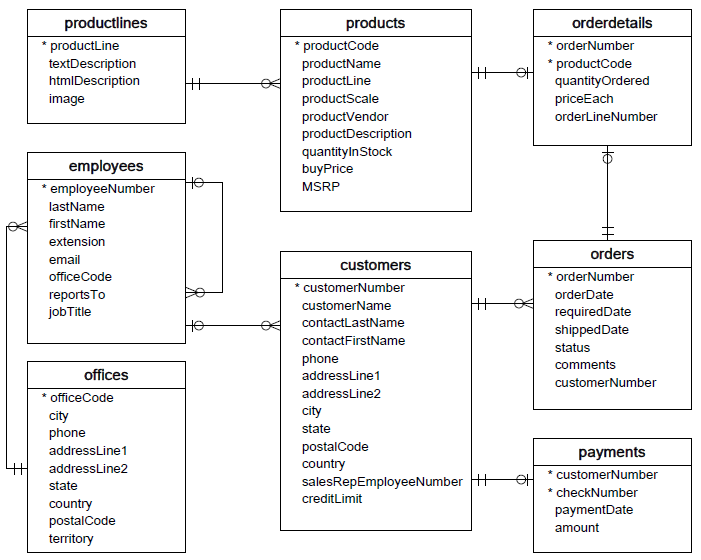
\includegraphics[width=0.6\columnwidth]{img/classicmodels.png}
\end{center}
L'url per scaricarlo: \url{https://www.mysqltutorial.org/getting-started-with-mysql/mysql-sample-database-aspx/}

\subsection{Istruzione SELECT}
\flushleft
\begin{lstlisting}[language = SQL]
SELECT attributo1 [, attributo2, ...]
FROM tabella1 [, tabella2, ...]
[WHERE condizione]
\end{lstlisting}
\begin{itemize}
\item $*$: vogliamo indicare tutti gli attributi
\item $FROM$: da che tabella
\item $WHERE$: quali ennuple, solo quelle dove è soddisfatta la condizione
\end{itemize}
\textcolor{blue}{Esempio}: mostra nome, prezzo di acquisto e di vendita dei modellini che costano meno di 75\$\\
\begin{lstlisting}[language = SQL]
SELECT productName, buyPrice, MSRP FROM products
WHERE MSRP < 75;
\end{lstlisting}

\subsection{Istruzione AS}
L'istruzione AS ha lo scopo di rinominare gli attributi\\
\begin{lstlisting}[language = SQL]
SELECT 	productName AS nomeProdotto, 
				productVendor AS nomeVenditore 
FROM products;
\end{lstlisting}

\subsection{Condizioni: Testo esatto}
\textcolor{blue}{Esempio}: Mostra tutti i dipendenti di nome 'Leslie'\\
\begin{lstlisting}[language = SQL]
SELECT * FROM employees
WHERE firstName = 'Leslie';
\end{lstlisting}
\paragraph{Virgolette singole o doppie?} è indifferente! Anche se lo standard ANSI dice singole\\
\textsl{Come posso inserire una virgoletta in una stringa?} Basta raddoppiarla.\\
\textcolor{blue}{Esempio}: Ci'ao lo scrivo come 'Ci''ao'

\subsection{Condizioni: Testo incompleto}
\textcolor{blue}{Esempio}: Mostra tutti i dipendenti il cui cognome finisce per 'son'\\
\begin{lstlisting}[language = SQL]
SELECT * FROM employees
WHERE lastName LIKE  '%son';
\end{lstlisting}
\begin{itemize}
\item \% : zero o più caratteri
\item \_ : esattamente un carattere
\item Per cercare il carattere \% uso $\backslash\%$
\item Per cercare il carattere \_ uso $\backslash\_$
\end{itemize}

\subsection{Intervalli}
Seleziona i valori compresi tra x e Y (inclusi)
\begin{lstlisting}[language = SQL]
SELECT ... FROM ...
WHERE colonna BETWEEN x AND y;
\end{lstlisting}

\subsection{Liste}
Controlla se il valore è presente in una lista di valori
\begin{lstlisting}[language = SQL]
SELECT ... FROM ...
WHERE colonna IN (val1, val2, ...);
\end{lstlisting}

\subsection{Gestire i NULL}
\begin{lstlisting}[language = SQL]
SELECT ... FROM ...
WHERE colonna IS NULL;
\end{lstlisting}

\subsection{Funzioni}
Per le \textbf{stringhe}:
\begin{itemize}
\item length()
\item reverse()
\item right()
\item trim()
\item \dots
\end{itemize}
Per \textbf{Data e Ora}:
\begin{itemize}
\item day()
\item year()
\item now()
\item month()
\item monthname()
\item \dots
\end{itemize}

\subsection{Ordinamento}
\#249


%----------------------------------------------
% FINE DOCUMENTO
%----------------------------------------------
\end{document}